\section{Features to be tested}
\begin{figure}[h!] 
\centering 
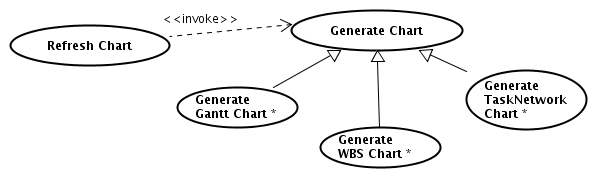
\includegraphics[width=0.7\textwidth]{desing_spec/GenerateChart.png}
\caption{spaccato tratto dal package \emph{Commons} del documento di analisi,
parte \emph{Use cases}}
\end{figure}
Verranno testati tutti gli use case espressi dalla figura tranne ``Refresh
Chart'' in quanto \`e stato riportato solo per favorire la comprensione del
contesto e perche la sua attivit\`a di costruire la \emph{UserOptionChoice} e
recuperare l'insieme dei \emph{Task} vengono testate nel documento
\footnote{make a test document for these use cases.}
\section{Raffinamento della strategia}

\section{Tests identification}

\section{Pass/fail criteria}